\section{Experimental Validation}
\label{Sec:Experiments}

This section discusses or tries to answer several key questions by
simulating the Trinity system described later.
Will Cerberus improve application performance by utilizing burst buffer nodes?
Will job demand on burst buffer effect Cerberus?
Why bother to model the job execution in 3 phases?
Can dynamic programming based optimization help Cerberus further
improve application performance?

\subsection{Simulation Settings}
We consider simulating the full Trinity super computer\cite{TrinitySystem}.
The number of compute nodes on Trinity is about 18,936,
e.g. 9,436 Intel Haswell nodes
and at least 9500 Intel Xeon Phi nodes.
There are 16 cores on each processor, thus totally 302,976 cores.
In the following experiments, we compare two identical system except that
IO nodes are replaced by the same number of burst buffer nodes.
Eventually Trinity plans to delivery up to 576 burst buffer nodes of 3.7 PB,
consisted of Trinity IO nodes with PCIe SSD card.
They are globally accessible as intermediate storage and distributed among cabinets.
Sequential read/write between burst buffer nodes and compute nodes is 8.0 GB/s.
Bandwidth between CPU node and non-burst-buffer IO node is set to 2.5 GB/s.
Job trace is from ANL's Blue Gene Intrepid system
from January to September 2009\cite{JobTrace}.
We extract two critical fields from this jobs trace: running time and
number of cores user requested.
This trace contains 68,936 jobs but
only the first 1,185 jobs are considered in this section's simulation.
We patched 3 fields to each job's log entry: the amount of input data $data\_in$,
the total amount of written data for checkpointings $data\_run$
and the amount of output data $data\_out$.
We assume they follows uniform distribution with
lower boundary of 1 TB and upper boundary of 60 TB.
The patches 3 fields may or may not be used in scheduling,
depends on both the model of the jobs and the experiment scenario.


\subsection{Cerberus vs. 1-Phase Batch Scheduler}
\label{Sec:Sim:DirectIOvsBB}
In this section, we demonstrate that by utilizing burst buffer nodes,
job scheduler could improve the applications' performance.
Figure~\ref{Fig:DirectIOvsBBResponse} compares CDF of the response time of 1185 jobs.
When scheduler can allocate burst buffer to jobs (denoted as Plain BB),
all jobs finish in 358,000 seconds counting from their submission time.
However, the worst case in system without burst buffer (denoted as Direct IO) is catastrophical.
There are jobs that takes almost 1,450,000 seconds to finish,
which is 4.05 times slow as the most non-responsive job
in system equipped with burst buffer.
In average case, more than 90\% of the jobs scheduled by Cerberus
response faster than 1-Phase Batch scheduler.
The improvement mainly comes from the difference of IO operation efficiency between
traditional IO nodes and burst buffer nodes.
There are only less than 10\% of the jobs response quicker without needing burst buffer.
Figure~\ref{Fig:DirectIOvsBBWait} reveals the total waiting time for both cases.
Notice that system without burst buffer only request compute nodes.
This means the waiting time is exactly the duration
from its submission to actual starting running.
The difference of worst case waiting time is drastic.
Without burst buffer nodes, job's wait duration in worst case is 6.41 times
slow as the worst one on systems with burst buffer;
the upper bound of waiting duration for burst buffer systems is about 210,000 seconds.
The reason is more than just bandwidth increment
for in our simulation setting $BW_{bb} / BW_{io}=3.2$.
More implicit reason is that because of burst buffer's better ability to
absorb checkpoint operations and data moving in/out,
the execution pipeline of job series is significantly speed up.
Statistically, 80\% jobs waited less time, thus response faster,
if they can access burst buffer.


Using the collected completion time, we can calculate system's throughput over time sequence.
Figure~\ref{Fig:DirectIOvsBBThroughput} shows the number of tasks finished
in a fixed time unit (500 seconds) for system using burst buffer nodes and not.
It totally takes 1,448,512 seconds for the system without burst buffer nodes to
server all 1185 jobs.
The last job is job \#1150, which requested 4096 cores and 59 TB data space.
It starts at 380 seconds but waited 1,341,696 seconds.
In contrast, when system installed burst buffer nodes,
it accomplishes the same 1185 jobs in 357,586 seconds.
Job \#1150 is the second last job finished, but both its waiting time and response time
are significantly reduced, 202853 and 256866 seconds respectively.
As indicated by the bar chart,
the ratio of average throughput between two systems is a little larger than 4, namely 1.662 to 0.411.
This approximately coincides with the 4-time worst-case response speedup,
made possible due to burst buffer equipments.

\begin{figure*}[!t]
        \centering
        \subfloat[Job Response Time] {
                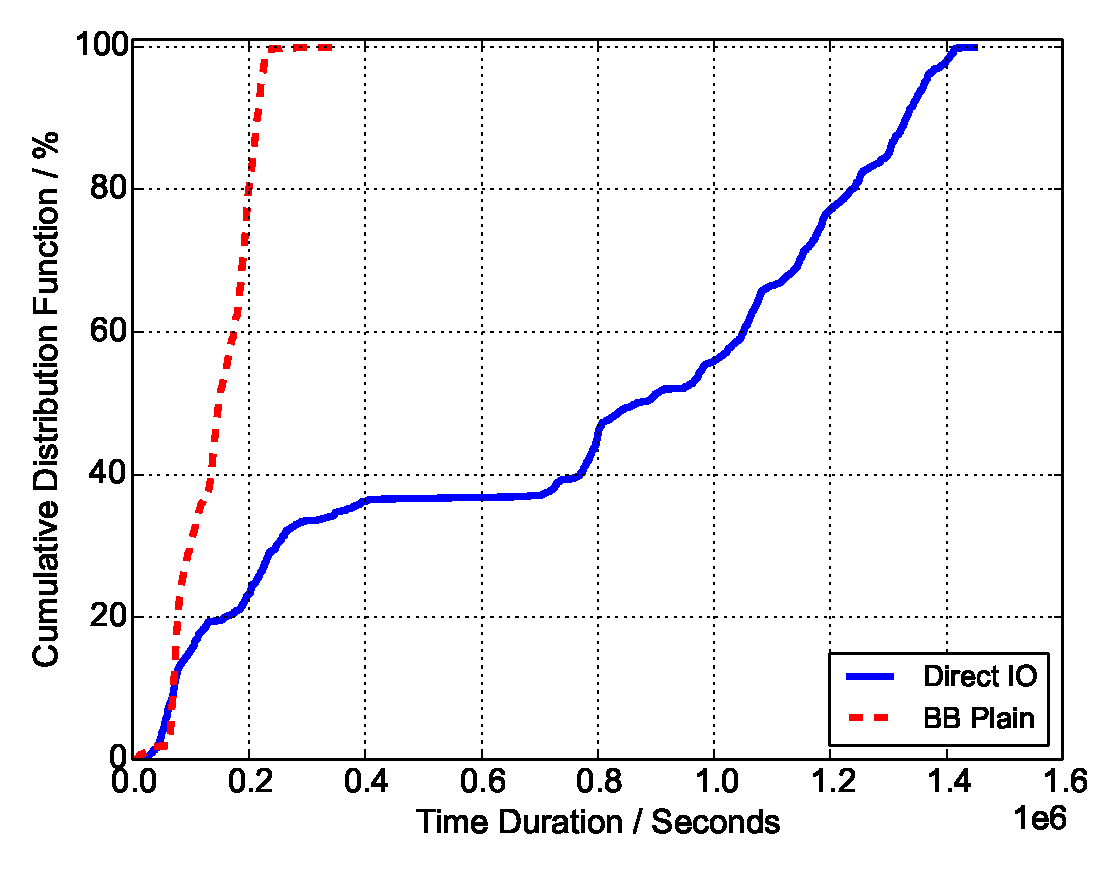
\includegraphics[width=3.2in]{DrawDirectIOvsBB/1000jobs_direct_vs_bb_response}
                \label{Fig:DirectIOvsBBResponse}
        }
        ~
        \subfloat[Job Wait Time] {
                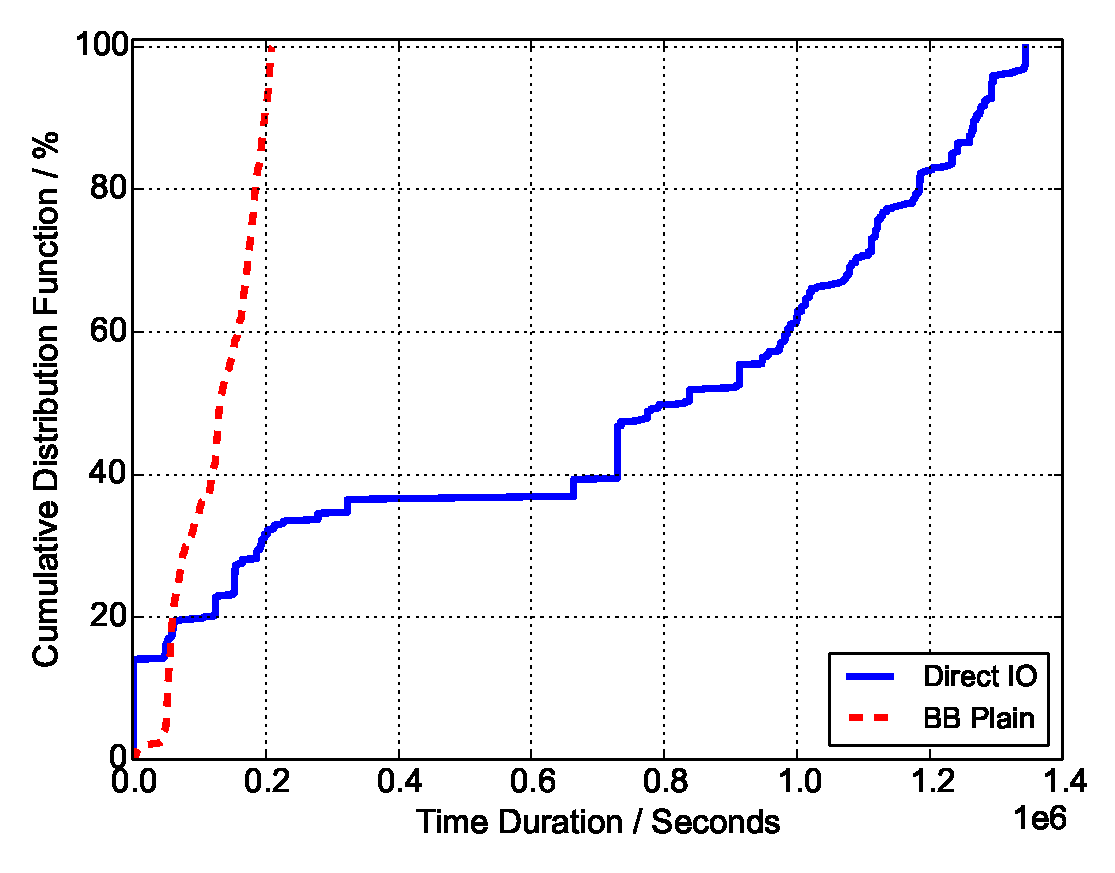
\includegraphics[width=3.2in]{DrawDirectIOvsBB/1000jobs_direct_vs_bb_wait}
                \label{Fig:DirectIOvsBBWait}
        }
        \caption{Performance of 1185 Applications: IO Node Only System vs. Burst Buffer System}
        \label{Fig:DirectIOPerformance}
\end{figure*}


\subsection{Cerberus vs. Demand Granularity}
In this section we validate our 3-phase model.
Applications are benefited when scheduler dividing jobs into 3 separated phases and 
scheduling are based on corresponding burst buffer demand in each phase.
This suggests that user should provide burst buffer demand as granular as possible.

In Figure~\ref{Fig:3Pvs1PResponse}, we plot 3 different scheduling results by 3 FCFS scheduler.
Jobs in the first case, denoted as Direct BB, are modeled as just 1 phase.
All users just provides a general burst buffer demand throughout entire application life time.
We assume this demand is the $\max \{data\_in, data\_out, data\_run\}$.
This is the traditional scheduling scheme except job has additional
burst buffer demand and scheduler must subject to burst buffer capacity constraint.
Jobs in the second and third cases have 3 phases and are scheduled by Cerberus.
However, in the second case, denoted as Plain BB 1D, Cerberus only knows
the overall burst buffer demand, same as the information in case 1.
In the 3rd case, named Plain BB 3P,
users kindly provided all the burst buffer demand in all 3 phases.
This is the same case as in section~\ref{Sec:Sim:DirectIOvsBB}
when we demonstrating burst buffer is beneficial.
We simulate the 3 cases with the same generated random data volume sequence.
For 1-phase-modeled jobs, scheduler will make decision
based on $\max \{data\_in, data\_out, data\_run\}$
since we assume user will only tell the upper bound of its application's demand.
However, in simulation, we use the generated data amount as the same as 3-modeled jobs.
%Response time of system without burst buffer devices are also plotted for comparison.

%Unsurprisingly, jobs' response time is improving as long as they could utilizing burst buffer.
Let's compare scheduling results of 1-phase and 3-phase D,
both of which only have rough data information of application.
More than 60\% of the 3-phase-modeled jobs finish faster than 1-phase-modeled jobs.
The longest 3-phase-modeled job takes 395,211 seconds to finish
while the slowest 1-phase-modeled job needs about 581,000 seconds to finish.
The improvement is about 38.69\% for the worst case.
The reason of such improvement is as follows.
For the 1-phase-modeled jobs, burst buffer nodes will be exclusively taken by scheduled jobs
throughout their lifetime.
In contrast, each time a 3-phase-modeled job finish inputing, running or outputing,
Cerberus will reclaim burst buffer and CPU resources.
This gives Cerberus more opportunity to schedule the system resources.
At last, when comparing the case of 3-phase IRO with 3-phase D,
we find another advantage of our 3-phase model.
If benign users can provide finer-grain information of data/IO demand,
Cerberus can programme each queue separately and get better scheduling result.
In our simulation, when Cerberus knows more about application's demand in different phases,
the worst absolute response time is less than 358,000 seconds.
This is 9.42\% improvement to 3-phase-modeled jobs
when Cerberus only knows the upper bound of data demand,
38.38\% better than the slowest 1-phase-modeled job.
In average case, 80\% of the 3-phase-modeled jobs scheduled by Cerberus
finish earlier than 1-phase-modeled jobs,
on the same condition that the same amount of burst buffer nodes are available to applications.
Meanwhile, more than 90\% of the jobs takes less time if user specifies data usage demand
at each phase to Cerberus.

We can reason about why Cerberus's scheduling result is better than
naively integrating batch scheduler with burst buffer constraint
by looking at the detailed waiting time.
There are 3 queues in Cerberus;
correspondingly we have 3 kinds of waiting for jobs in Cerberus.
Figure~\ref{Fig:3Pvs1PWaitIn} shows the time job spend in inputing queue,
Figure~\ref{Fig:3Pvs1PWaitRun} the time job spend in running queue,
Figure~\ref{Fig:3Pvs1PWaitOut} the time job spend in outputing queue.
For 1-phase scheduler, there is just one queue;
therefore the waiting time in Figure~\ref{Fig:3Pvs1PWaitIn}~Figure~\ref{Fig:3Pvs1PWaitOut}
are all in fact the total waiting time.
Comparing the total waiting time shown in Figure~\ref{Fig:3Pvs1PWait}
to waiting time in different queues,
we see that jobs did not spend much time in either input queue $Q_I$ or output queue.
To be specific, the upper bounds of time spent in input queue are
$<$ 10\% and $<$ 20\% of the total waiting time in the case of 1-phase scheduler
for 3-phase D and 3-phase IRO respectively;
the upper bounds of time spent in output queue $Q_O$ are
less than 5\% of the total waiting time of 1-phase-scheduler case
for both 3-phases cases.
As for the time waiting for running, the corresponding upper bound percentages
are 30\% and 40\% approximately.
The difference of waiting time among 3 cases results in the different
response performance.


Figure~\ref{Fig:3Pvs1PThroughput} describes system throughput of these three different scenarios.
It helps us examine the performance of the scheduling in time sequence.
For 1-phase-modeled job, we can see an obvious `throughput gap'
from 180,000 second to 250,000 second approximately.
This is the result of too aggressive scheduling at the beginning.
For the case of 3-phase D, throughput also starts provocatively,
but not as provocatively as 1-phase scheduling case;
it is then calmed due to frequent resource release,
indicated by multiple crests and troughs from 0 to 400,000 seconds.
The 3-phase IRO runs counter to the both previous cases.
Even though beginning with throughput trough,
Cerberus manages to make the system having high throughput from 50,000 to 250,000 seconds,
during which system can achieve throughput around 10 to 12 per 500 seconds. 
In average, the throughput of 3-phase IRO case is 1.662 jobs / 500 seconds.
It is 62.15\% higher than the Direct BB case (1.025 jobs / 500 seconds) and
11.10\% higher than the Plain BB 1D case (1.496 jobs / 500 seconds).
We believe this validates the indispensable 3 phase job model and
the necessity that user provides data capacity demand for each phase.


\begin{figure}[!t]
        \centering
        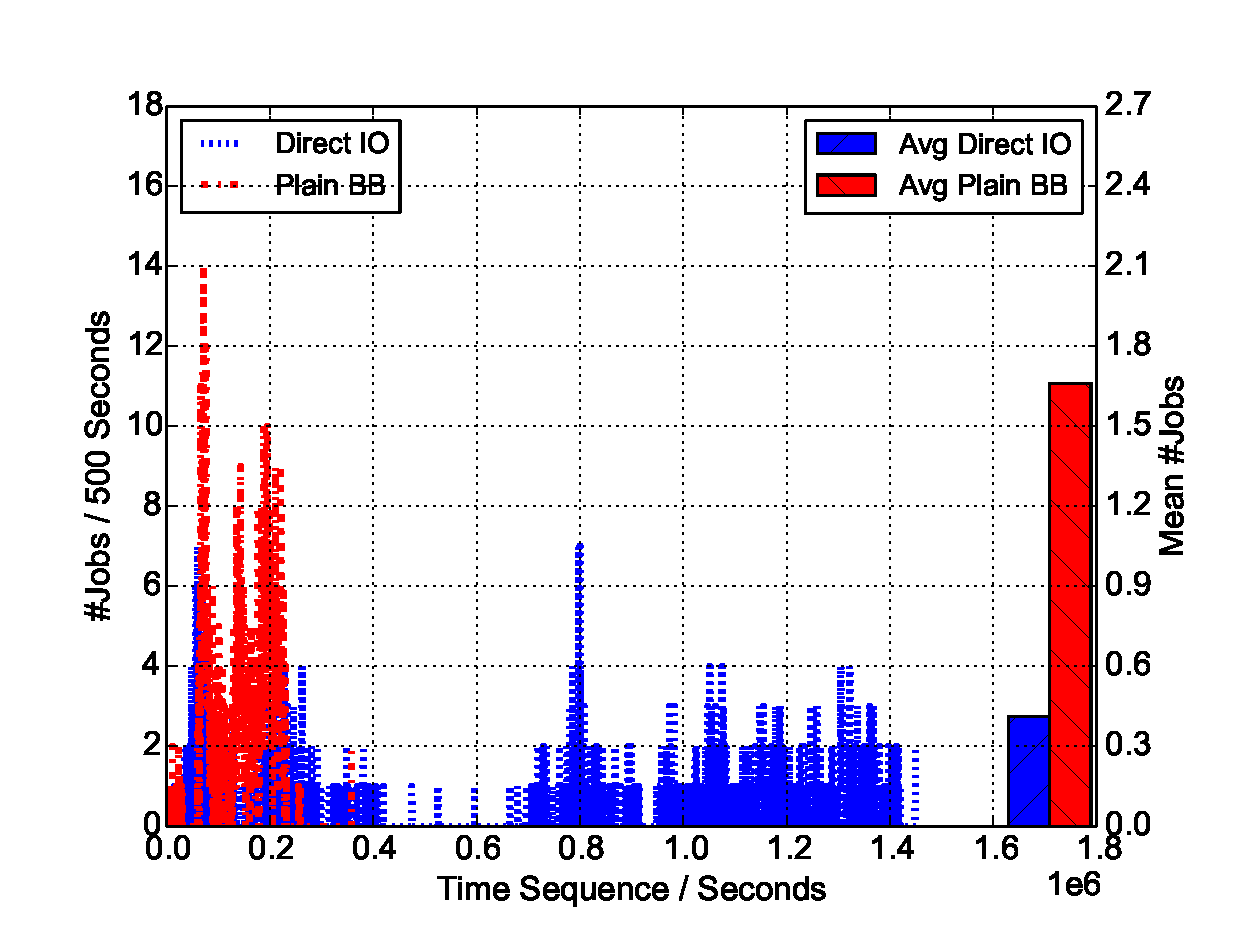
\includegraphics[width=3.2in]{DrawDirectIOvsBB/1000jobs_direct_vs_bb_throughput}
        \caption{System Throughput, IO Node Only vs. Burst Buffer System}
        \label{Fig:DirectIOvsBBThroughput}
\end{figure}

\begin{figure*}[!t]
        \centering
        \subfloat[Job Response Time] {
                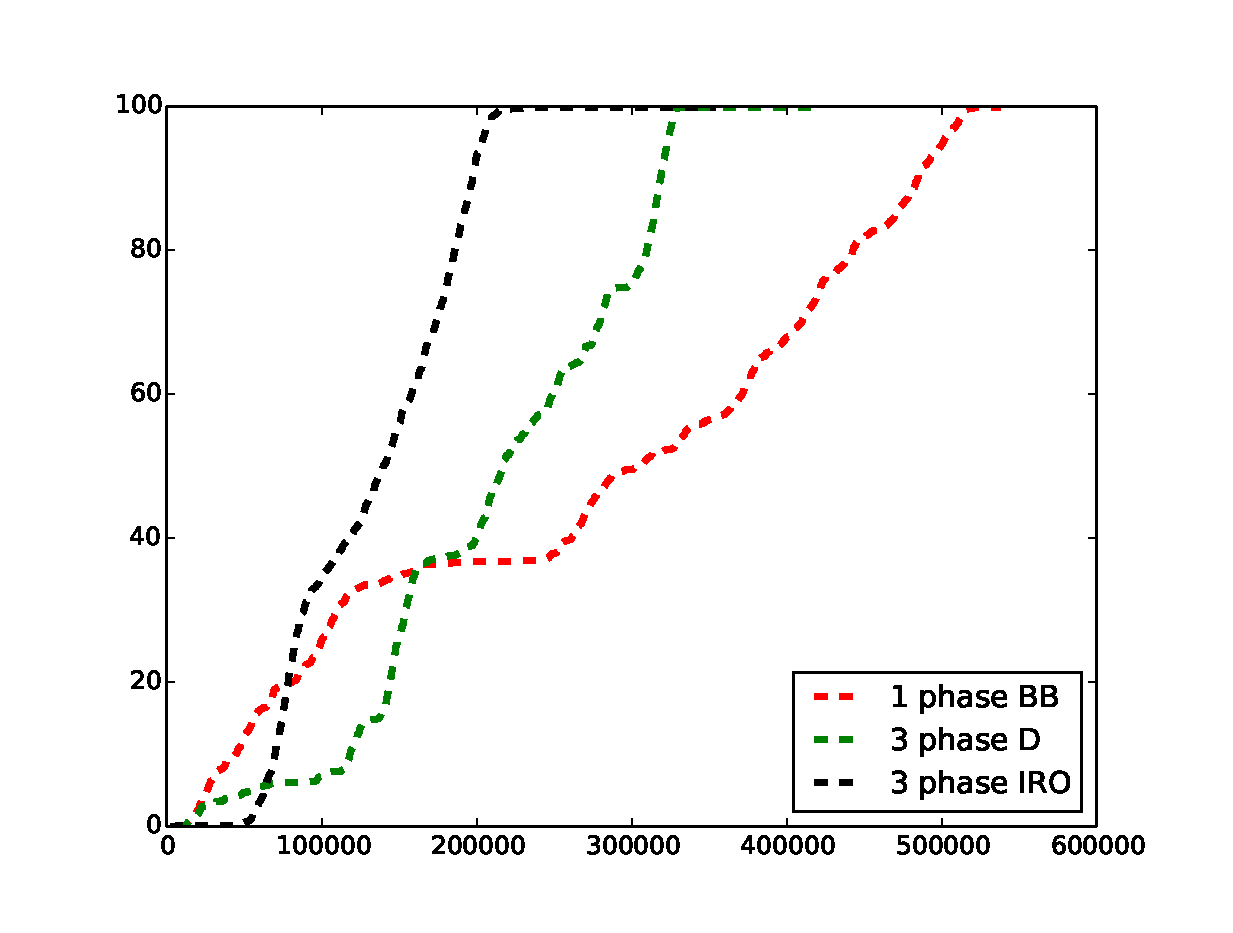
\includegraphics[width=3.2in]{Draw3Pvs1P/1000jobs_3p_vs_1p_response}
                \label{Fig:3Pvs1PResponse}
        }
        ~
        \subfloat[Job Wait Time] {
                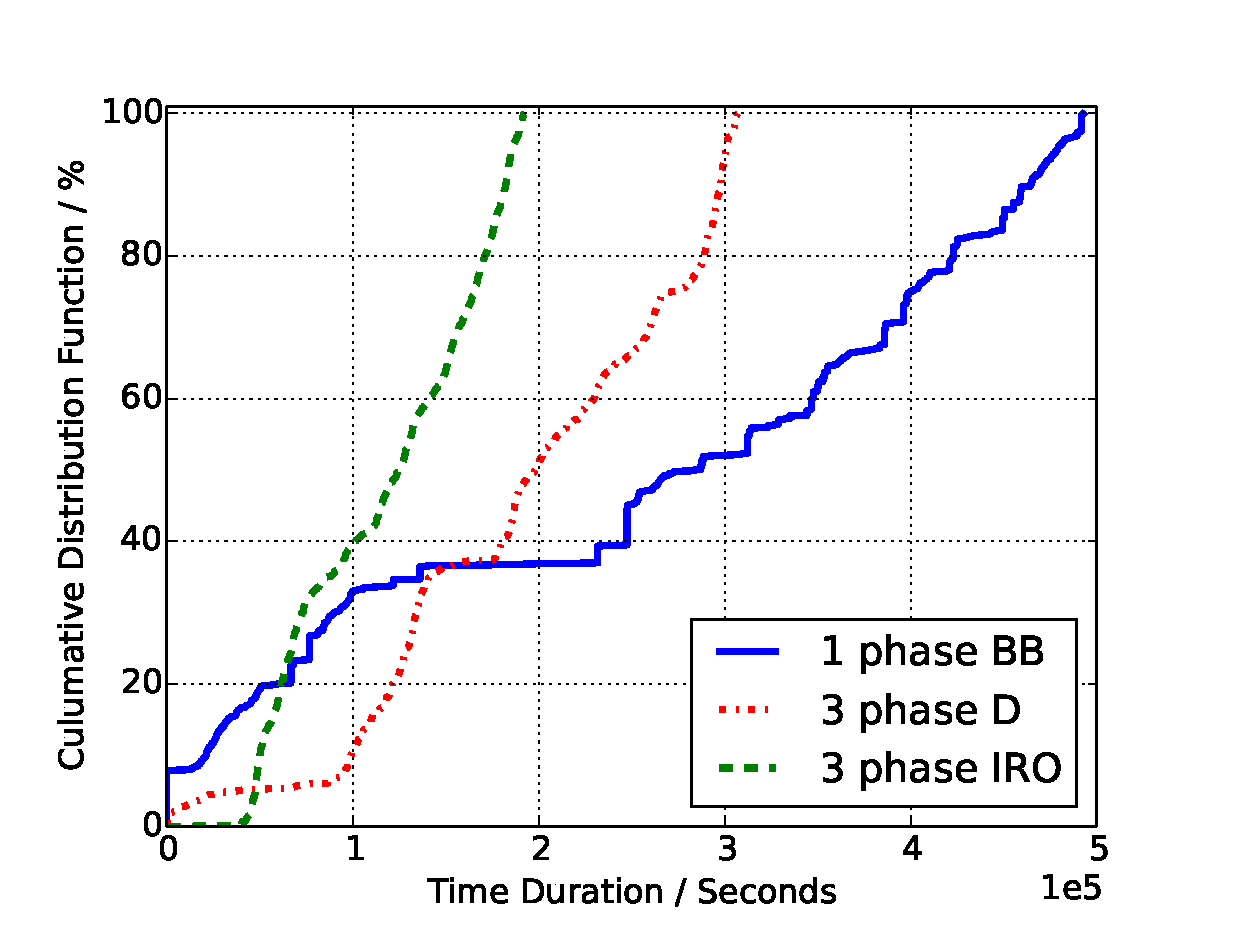
\includegraphics[width=3.2in]{Draw3Pvs1P/1000jobs_3p_vs_1p_wait}
                \label{Fig:3Pvs1PWait}
        }

        \subfloat[Job Wait Input Time] {
                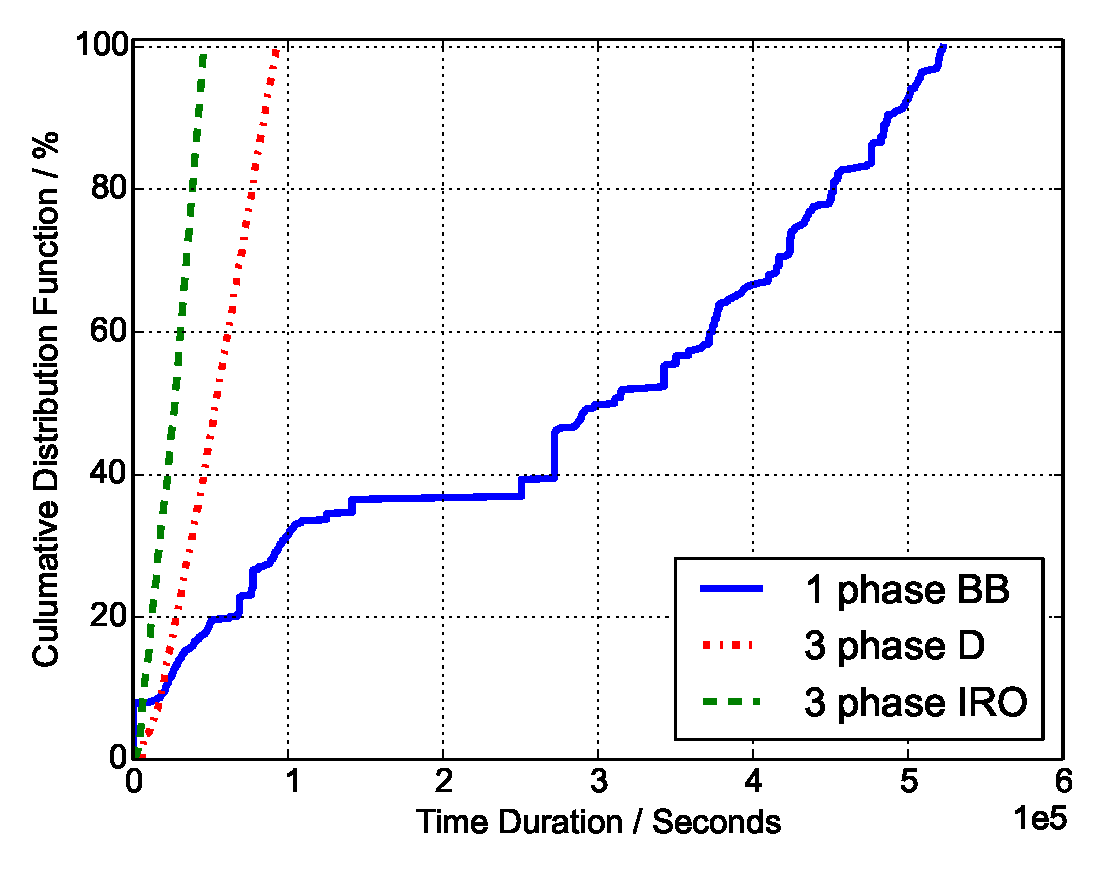
\includegraphics[width=2.3in]{Draw3Pvs1P/1000jobs_3p_vs_1p_wait_in}
                \label{Fig:3Pvs1PWaitIn}
        }
        ~
        \subfloat[Job Wait Run Time] {
                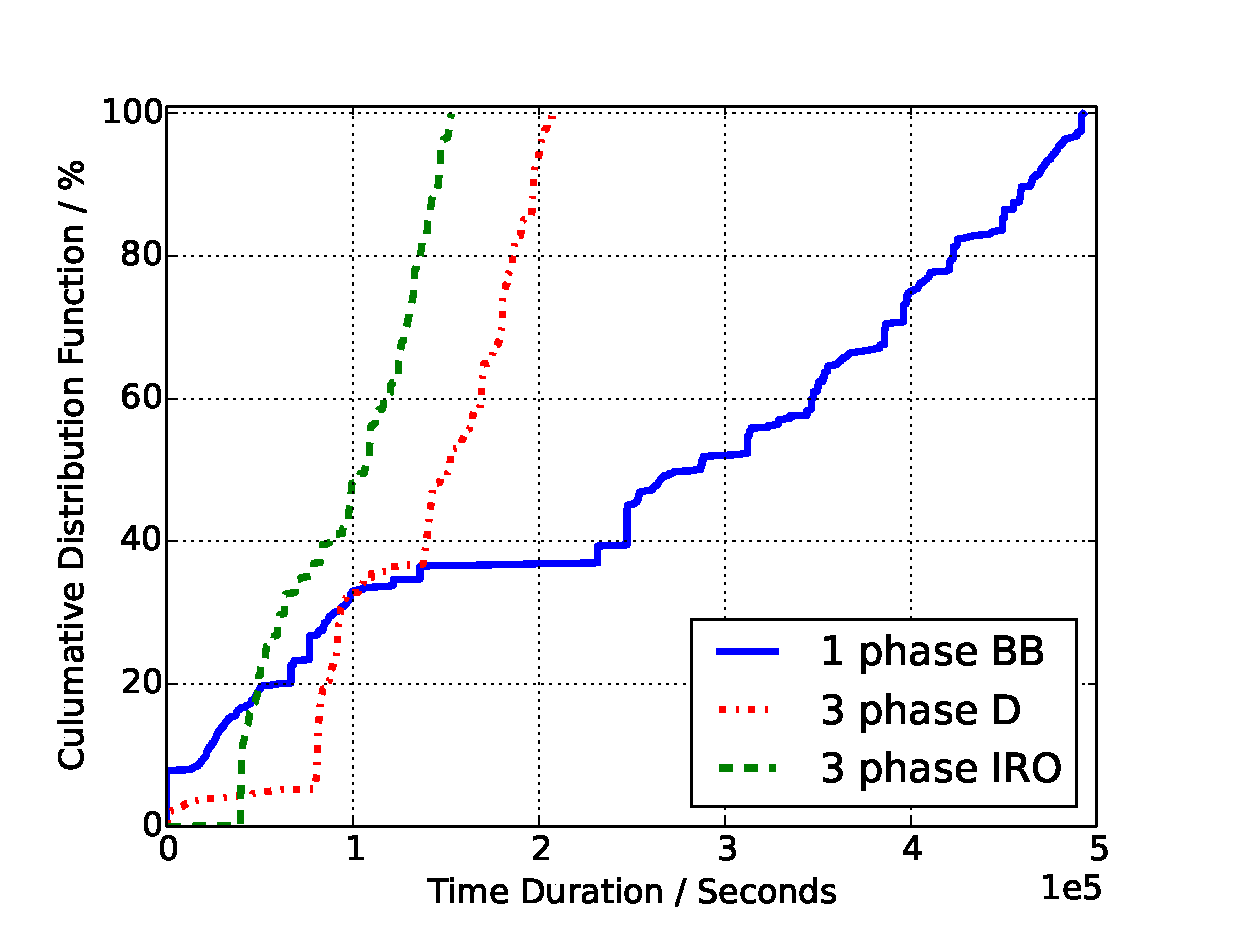
\includegraphics[width=2.3in]{Draw3Pvs1P/1000jobs_3p_vs_1p_wait_run}
                \label{Fig:3Pvs1PWaitRun}
        }
        ~
        \subfloat[Job Wait Output Time] {
                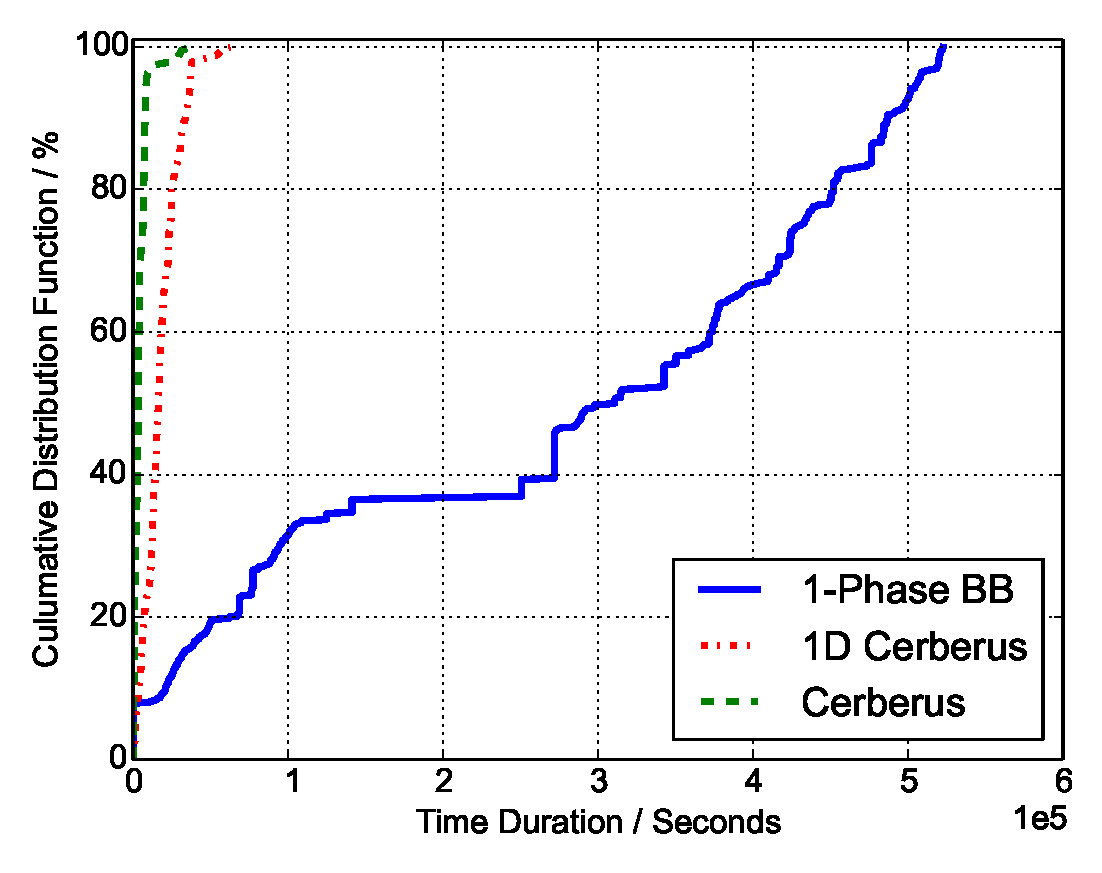
\includegraphics[width=2.3in]{Draw3Pvs1P/1000jobs_3p_vs_1p_wait_out}
                \label{Fig:3Pvs1PWaitOut}
        }
        \caption{Performance of 1185 Applications: 1 Phase Model vs. 3 Phase Model}
        \label{Fig:3Pvs1PPerformance}
\end{figure*}


\subsection{Cerberus vs. Cerberus with Optimization}
If we consider optimizing either burst buffer's data throughput or the parallelism across jobs,
dynamic programming based job scheduler can further reduce jobs' wait time.
We plot in Figure~\ref{Fig:DPvsFIFOResponse} the resulting response time of
three version of Cerberus scheduler differs in
how they handle jobs in their queues (input queue, run queue, and output queue).
The first scheduler uses naive first come first serve (FCFS) policy.
Whoever at the front of queue are considered favorably.
The second and third version treat jobs in run queue identically.
They choose jobs according to the optimization solution
given by Equation~\ref{Equ:MaxProductRecursion}
However, they treat jobs in the input queue and output queue differently.
The second version will select these jobs in its queue so that
volume of to be transferred data is maximized.
The dynamic programming recursion is Equation~\ref{Equ:MaxTransferDataRecursion}
The third version of Cerberus tries to optimize the number of jobs,
subjecting to burst buffer volume constraint by Equation~\ref{Equ:MaxTaskNumberRecursion}.

As indicated by Figure~\ref{Fig:DPvsFIFOResponse}, response time of
jobs scheduled by both Cerberus version 2 and 3 are reduced.
The most non-responsive job for both Cerberus Max-BB and Max-Task is job \#445,
taking 325,753 and 316,157 seconds respectively.
In contrast, job \#445 takes 357,206 seconds to finish when Cerberus using FCFS.
This is 9.66\% slower than Max-BB and 12.98\% slower than Cerberus V3.
When we consider the overall response time of entire job set,
we see more than 75\% of the tasks response faster when we choose jobs according to
optimization result.
The scheduling results of Cerberus V2 and V3 are fairly closed to each other.
In this simulation, 70\% of the jobs could get better response time
if we maximizing number of parallelable tasks,
versus maximizing transferred data.
The time duration application waits for running,
or the time application spend in running queue,
is plotted in Figure~\ref{Fig:DPvsFIFOWaitRun}.
We can see that in both optimization cases, Cerberus hold a couple of jobs waiting
in its running queue for a very long time,
even longer than the FCFS case.
We figure out the reason of this long delay once we examine the detail of these jobs.
First they are submitted at early middle phase.
Job \#435 waits 206,914 seconds in the maximizing burst buffer usage case;
job \#438 waits 205,375 seconds in the case of maximizing number of tasks.
Second, these jobs are requesting huge amount of compute nodes (163840 cores)
but comparably less burst buffer (7 TB for job \#435 and 8 TB for job \#438)
The third and the most important reason is that there are jobs requesting similarly
large number of cores but request less running time and larger amount of burst buffer.
For example, job \#434 also requests 163840 cores
but its request running time is just 3600 seconds;
job \#434 also requests 45 TB burst buffer.
As a result, Cerberus, according to Equation~\ref{Equ:MaxProductRecursion},
favors the jobs with less request time but larger burst buffer demand.
This is interesting because it is a potential flaws in the optimization-based policy:
given the user knows the optimization objective of our scheduler,
it is possible for a user to cheat scheduler by lying about her demand.
In other words, our optimization scheme, even though providing performance enhancement
for the waiting time of 80\% jobs, is not strategy-proofness\cite{Ghodsi:NSDI:2011}


We can see in Figure~\ref{Fig:DPvsFIFOThroughput} the throughput of system
when scheduled by 3 different versions of Cerberus.
For optimal Cerberus, job \#445 decides the finishing time of all 1185 jobs.
That is 326,133 seconds for Cerberus when it maximizing data throughput
and 316,590 seconds for Cerberus when it maximizing parallelable tasks.
The plain Cerberus, scheduling jobs in queue with FCFS policy,
makes system ends its last job, also job \#455, at 357,586 seconds.
The worst case completion improvement to FCFS-style Cerberus is
8.80\% for max-BB-style Cerberus and 11.46\% for max-number-task-style Cerberus.
When we look at the time sequence of throughput,
we found the peak value 16 jobs / 500 seconds obtained Cerberus
when maximizing the number of parallel tasks being able to run.
The alternative optimization method, maximizing burst buffer's usage,
could achieve 14 jobs / 500 seconds before 20000 seconds.
The peak throughput of FCFS policy is 13 jobs / 500 seconds around 50000 seconds.
Mean throughputs of these 3 scheduling methods are drawn
as bar chart in Figure~\ref{Fig:DPvsFIFOThroughput}.
Comparing with FCFS Cerberus, max-BB version achieves
10.41\% higher average throughput (1.835 jobs / 500 seconds)
while max-number-task version gives 13.24\% improvement (1.882 jobs / 500 seconds),
that is, extra 2.83\% enhancement to max-BB version.

\begin{figure}[!t]
        \centering
        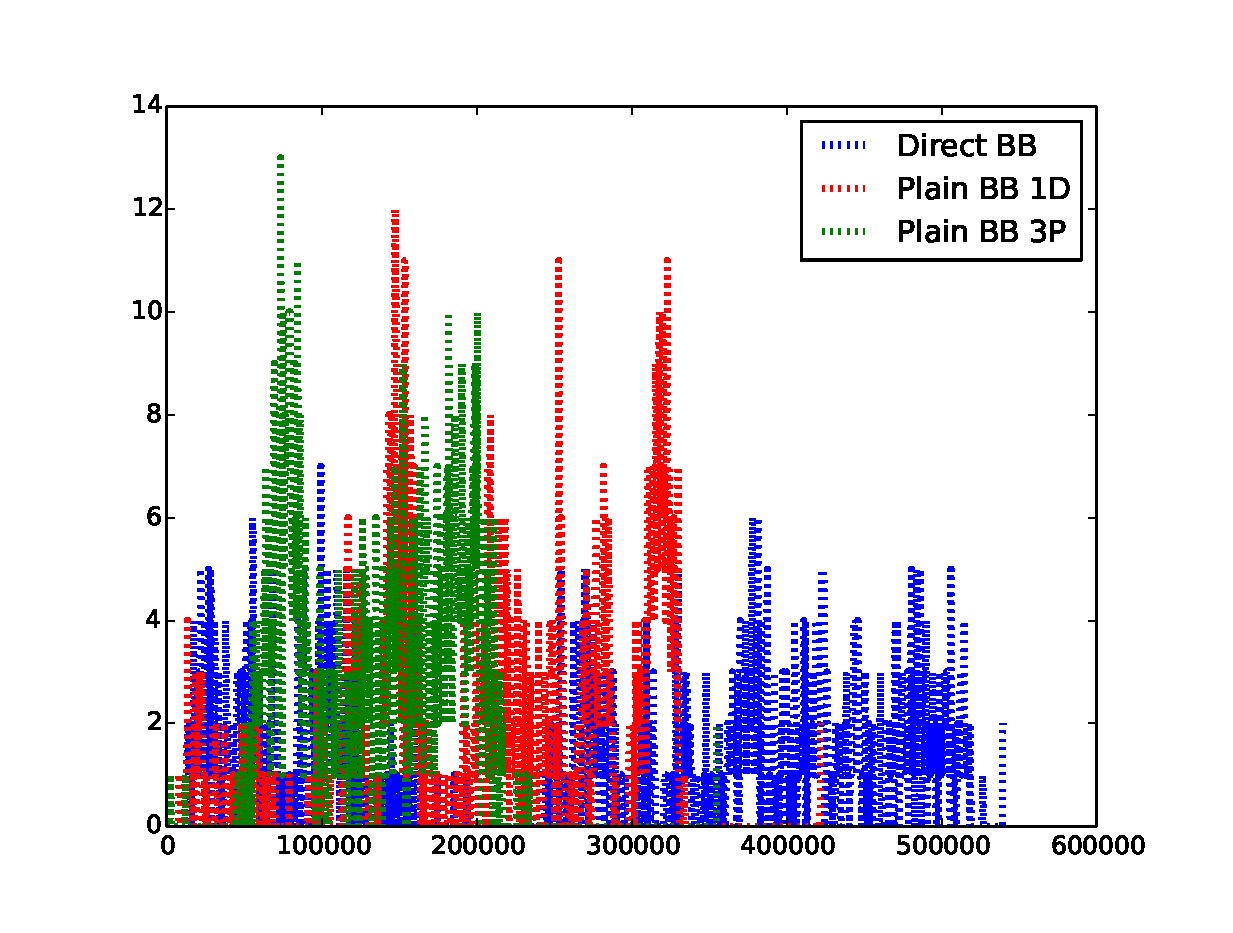
\includegraphics[width=3.2in]{Draw3Pvs1P/1000jobs_3p_vs_1p_throughput}
        \caption{System Throughput, 1 Phase Model vs. 3 Phase Model}
        \label{Fig:3Pvs1PThroughput}
\end{figure}

\begin{figure*}[!t]
        \centering
        \subfloat[Job Response Time, Dynamic Programming vs. FCFS] {
                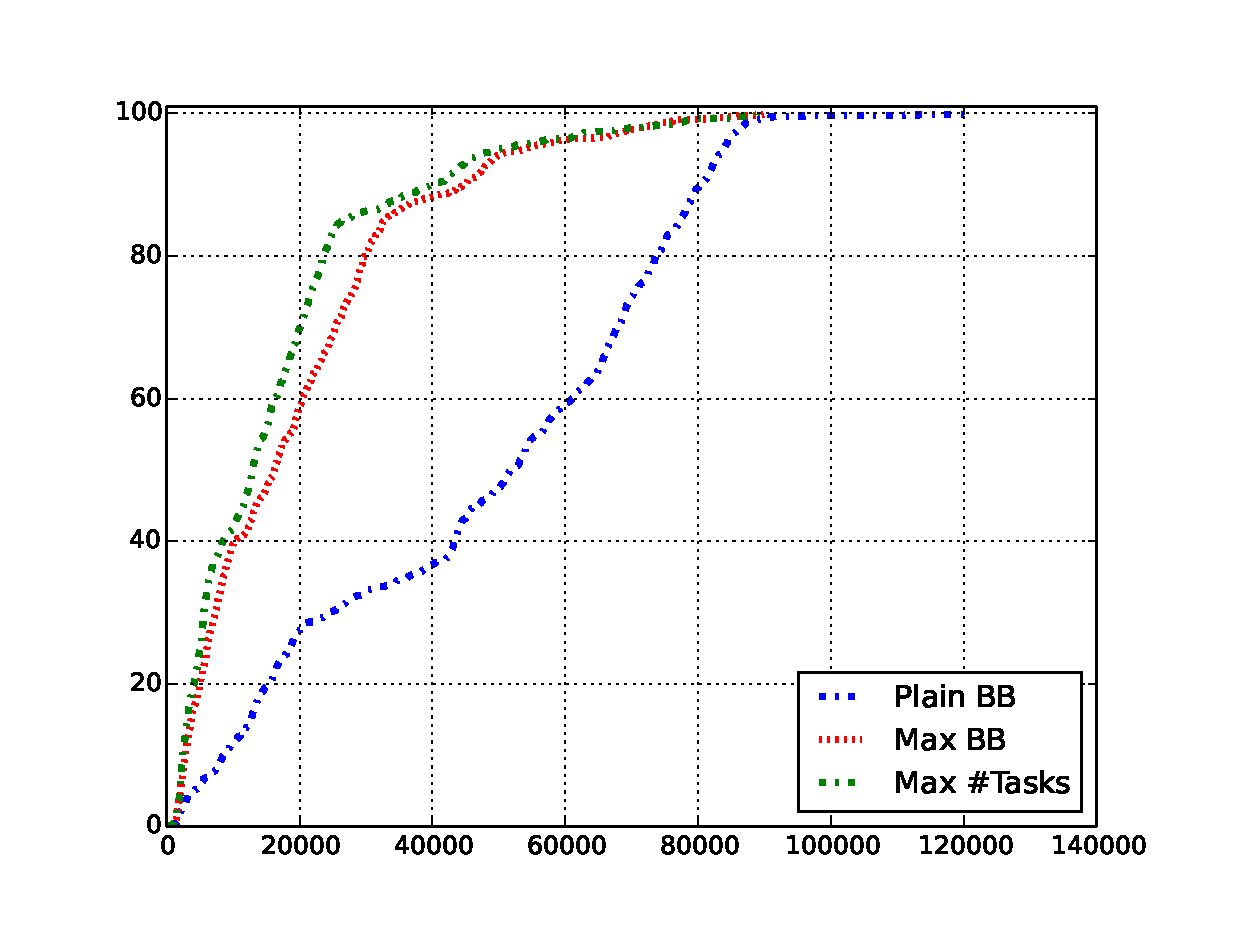
\includegraphics[width=3.2in]{DrawDPvsFIFO/1000jobs_dp_vs_fifo_response}
                \label{Fig:DPvsFIFOResponse}
        }
        ~
        \subfloat[Job Wait Run Time] {
                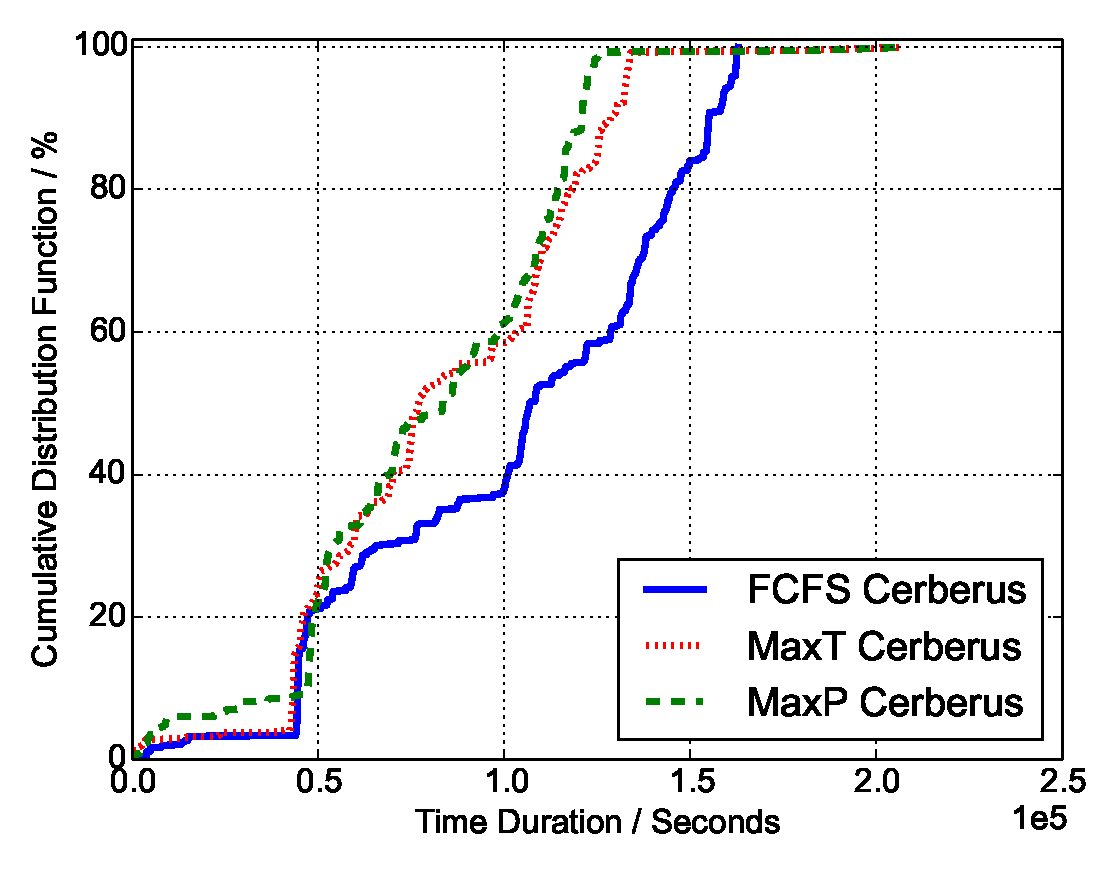
\includegraphics[width=3.2in]{DrawDPvsFIFO/1000jobs_dp_vs_fifo_wait_run}
                \label{Fig:DPvsFIFOWaitRun}
        }
        \caption{Performance of 1185 Applications: Dynamic Programming vs. FCFS}
        \label{Fig:DPvsFIFOPerformance}
\end{figure*}

\begin{figure}[!t]
        \centering
        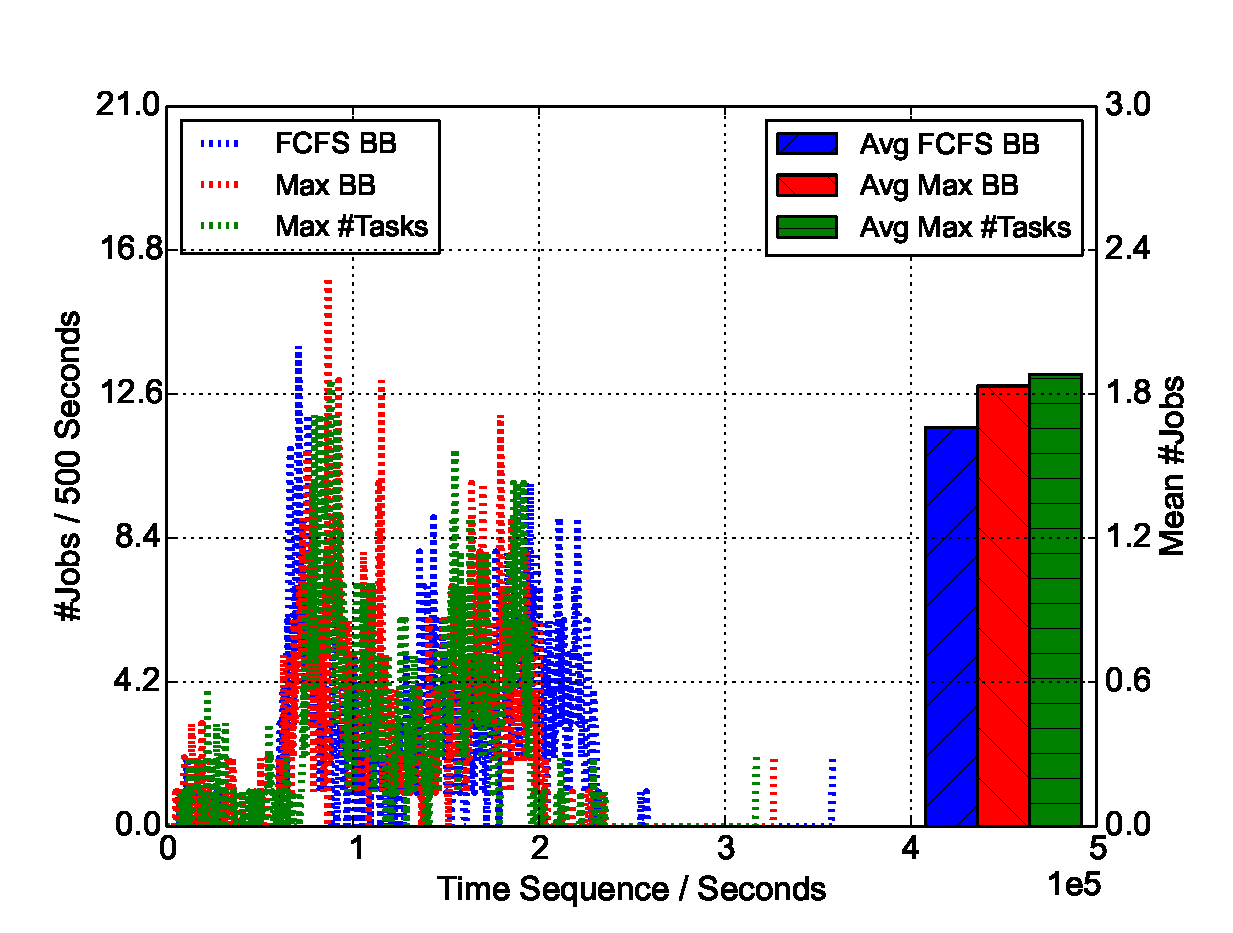
\includegraphics[width=3.2in]{DrawDPvsFIFO/1000jobs_dp_vs_fifo_throughput}
        \caption{System Throughput, Dynamic Programming vs. FCFS}
        \label{Fig:DPvsFIFOThroughput}
\end{figure}

\begin{table}[!t] 
        \renewcommand{\arraystretch}{1.3}
        \caption{Time Consumption in Dynamic Programming}
        \label{Tab:OptimizationTime}
        \centering
        \begin{tabular}{l|c|c|c}
                \hline
                Scheduling Policy Used & FCFS & Max BB & Max \#Task \\
                \hline
                \hline
                Simulation Time / seconds & 6.59 & 246.87 & 207.42 \\
                Optimization Time / seconds & 0 & 241.11 & 201.75 \\
                Total Number of Optimizations & 0 & 8702 & 9114 \\
                \hline
        \end{tabular}
\end{table}

\begin{table}[!t] 
        \renewcommand{\arraystretch}{1.3}
        \caption{Time Consumption in Dynamic Programming}
        \label{Tab:OptimizationTime}
        \centering
        \begin{tabular}{l|c|c}
                \hline
                Scheduler Policy Used & Max BB & Max \#Task \\
                \hline
                \hline
                Simulation Run Time / seconds & 246.87 & 207.42 \\
                Optimization Run Time / seconds & 241.11 & 201.75 \\
                Total Number of Optimizations & 8702 & 9114 \\
                \hline
        \end{tabular}
\end{table}


